\documentclass[tikz]{standalone}
\usepackage{pgfplots}
\usepackage{tikz}
\usepackage{xcolor}
\pgfplotsset{compat = 1.16}
\tikzstyle{format} = [rectangle, draw, fill = blue!20]
\usetikzlibrary{er,positioning}

\begin{document}
    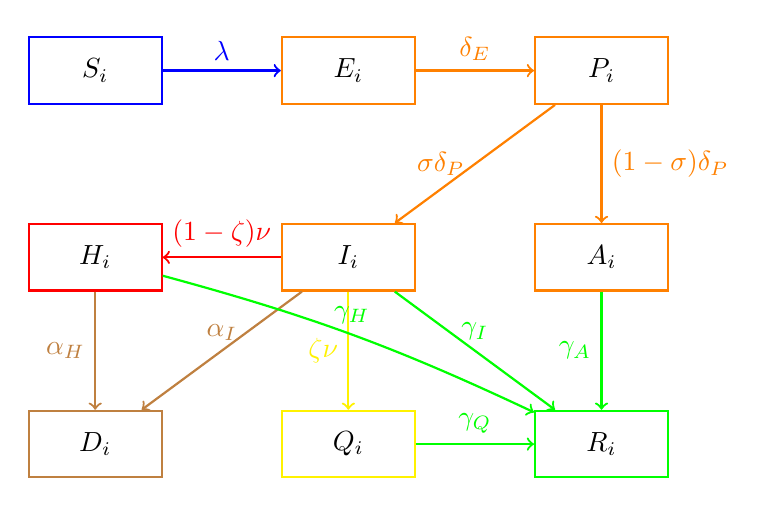
\begin{tikzpicture}[edge from parent/.style = {draw, -latex}]
        \node [entity, draw = blue, thick] (S) {$S_i$};
        \node [entity, draw = orange, thick] (E) [right = 1.5cm of S] {$E_i$};
        \node [entity, draw = orange, thick] (P) [right = 1.5cm of E] {$P_i$};
        \node [entity, draw = orange, thick] (I) [below = 1.5cm of E] {$I_i$};
        \node [entity, draw = orange, thick] (A) [below = 1.5cm of P] {$A_i$};
        \node [entity, draw = red, thick] (H) [below = 1.5cm of S] {$H_i$};
        \node [entity, draw = yellow, thick] (Q) [below = 1.5cm of I] {$Q_i$};
        \node [entity, draw = green, thick] (R) [below = 1.5cm of A] {$R_i$};
        \node [entity, draw = brown, thick] (D) [below = 1.5cm of H] {$D_i$};
        
        \path[->]
            (S) edge [blue, thick] node[above] {$\lambda$} (E)
            (E) edge [orange, thick] node[above] {$\delta_E$} (P)
            (P) edge [orange, thick] node[right] {$(1 - \sigma)\delta_P$} (A)
                edge [orange, thick] node[left] {$\sigma \delta_P$} (I)
            (I) edge [red, thick] node[above] {$(1 - \zeta)\nu$} (H)
                edge [brown, thick] node[above] {$\alpha_I$} (D)
                edge [yellow, thick] node[left] {$\zeta \nu$} (Q)
                edge [green, thick] node[above] {$\gamma_I$} (R)
            (A) edge [green, thick] node[left] {$\gamma_A$} (R)
            (H) edge [bend left = 5, green, thick] node[above] {$\gamma_H$} (R)
            (H) edge [brown, thick] node[left] {$\alpha_H$} (D)
            (Q) edge [green, thick] node[above] {$\gamma_Q$} (R);
    \end{tikzpicture}
\end{document}